\section{Functional Requirements}

\subsection{R1: Allow any citizen of legal age, as a visitor, to register on the mobile phone app or the web app and to become a user by providing a document}
\begin{itemize}
    \item The system must allow the visitor to provide credentials and personal data
    \item The system must verify the correspondence between the ID number provided by the visitor and their personal information
    \item The system must allow the visitor to verify the account with an e-mail or SMS verification code
    \item The system must send a recap of registration to email of the visitor
    \item The system must verify that there are no other registered users or authorities with the same e-mail or ID number
    \item The user must accept users data privacy conditions to successfully register to the system
    \item A citizen can register to SafeStreets by providing their ID number
    \item The system must allow a user to register with an email and a password, that will be asked every time they log in
\end{itemize}

\begin{description}
    \item \label{scenario1} \textbf{Scenario 1} \newline
        Mario Rossi saw the advertisement of SafeStreets and decided to download the mobile application in order to be allowed to notify violations and improve safety of streets in his city. After
        opening the new app, he is asked to fill a form with all his personal information, full name, email address, mobile number, ID card and phone number. To proceed with his
        registration, after having filled all the form, including the users data privacy conditions, Mario clicks on the "Create account" button. The system verifies the correspondence between inserted personal data and the ID card information,
        and if the verification is positive, Mario is asked whether he prefers to confirm his registration by phone number or by email.
        He chooses the alternative he prefers, then he immediately receives the verification code on the medium he chose.
        He can confirm his registration by clicking on the verification code. The system then sends a recap to notify the positive outcome of registration. Mario is now a Registered
        User of SafeStreets; he can login to notify violations on the streets and is enabled to the use of all the functions for a basic user (not an authority) that the system provides.
    \item \textbf{Use case: Visitor registration on mobile phone}
    \begin{center}
        \begin{tabular}{|p{3cm}|p{7cm}|}
            \multicolumn{2}{c}{\textbf{Visitor Registration}} \\
            \hline
            \textbf{Name} & Registration to SafeStreets \\
            \hline
            \textbf{Actor} & Visitor \\
            \hline
            \textbf{Goals} & R1 \\
            \hline
            \textbf{Entry conditions} & The visitor must have downloaded the mobile phone application or the visitor must have accessed the web interface \\
            \hline
            \textbf{Event flow} &
            \begin{enumerate}
                \item The Visitor must fill all mandatory fields in the registration form
                \item The Visitor must click on the "Create account" button
                \item The system validate the provided data 
                \item The Visitor chooses how to confirm his registration (phone number/email) 
                \item The system sends the code on the visitor's chosen mode, mobile phone or email address
                \item The Visitor clicks on the confirmation code
                \item The system sends a recap of registration, as a positive outcome 
                \item The system saves the Visitor's data
            \end{enumerate} \\
            \hline
            \textbf{Exit conditions} & The Visitor has become a registered used \\
            \hline
            \textbf{Exceptions}
            & \begin{itemize}
                \item The Visitor is already registered
                \item The email is already registered
                \item The ID card is already registered 
                \item Visitor's data don't match with ID card data
                \item Some mandatory fields are not filled 
                \item The user is a minor
            \end{itemize} \\
            \hline
        \end{tabular}
    \end{center}
\end{description}

\begin{figure}[hbt!]
    \centering
    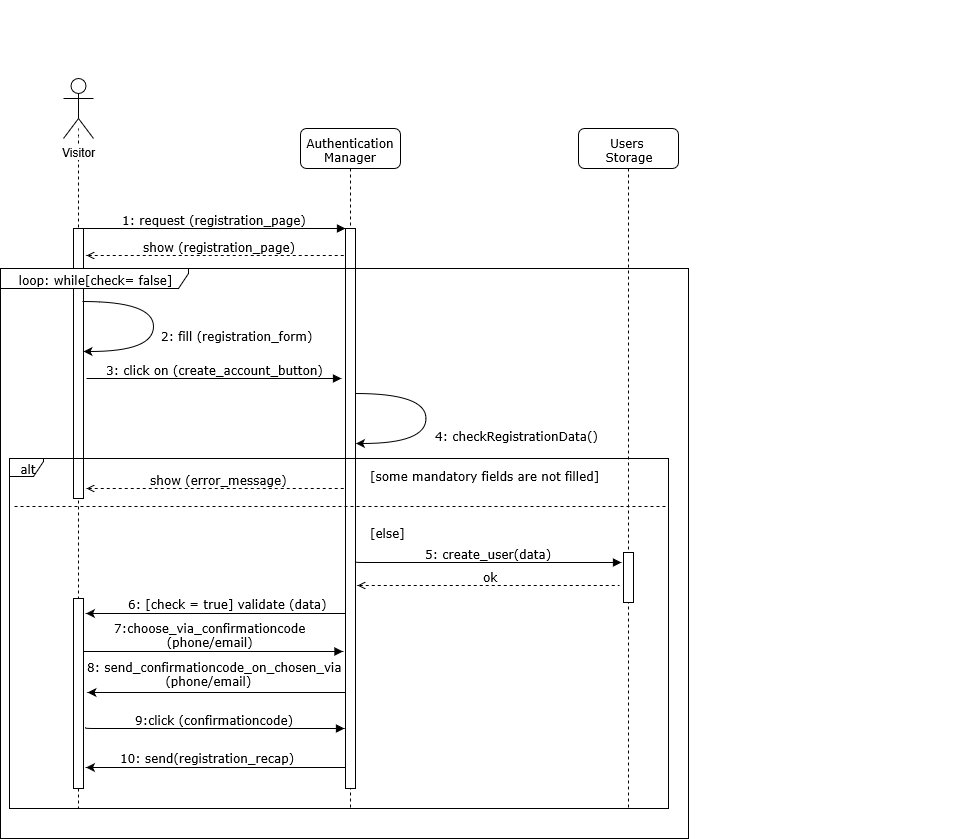
\includegraphics[width=\textwidth]{RASD_Images/SequenceDiagrams/1.jpg}
    \caption{\textit{Sequence diagram 1 - Visitor registration on mobile phone}}
\end{figure}

\subsection{R2: Allow a user to send pictures about street and parking violations}
\begin{itemize}
    \item A user can submit a picture to the system whenever they see a traffic violation
    \item SafeStreets analyses the image to read the license plate of the vehicle
    \item The user can manually attach the license plate to the image, to help the system with its validation
    \item The user must provide the type of violation, either selecting it from a list or manually typing it if it is not already in the system
    \item The user can help localizing the violation by inserting the name of the street where it occurred
\end{itemize}

\begin{description}
    \item \textbf{Scenario 2} \newline
        Mario Rossi is a user of SafeStreets, he has just finished working and he wants to go back home, but he is can't reach his car because of double parking. He waits for ten 
        minutes to see if the owner of the car is coming, but then decides to notify the violation. In order to notify the violation he must have logged into the mobile application, inserting his data, so he does; then he takes two pictures representing the violation, 
        then he clicks on the button to notify a violation, he inserts the position (Via Botticelli, Viale Romagna, 2, 20133 Milano MI), a brief description 
        of the violation and the two pictures. He is asked to select the category of the notified violation (Double-Row Parking), or to add it if it's still not present in the system.
        Then, he is asked to insert the license plate of the vehicle involved in the violation in the mobile application, he does, then the app verifies that it 
        corresponds to the license plate identified with the photograph.
    \item \textbf{Use case: User sends pictures on mobile phone to notify a parking violation}
    \begin{center}
        \begin{tabular}{|p{3cm}|p{7cm}|}
            \multicolumn{2}{c}{\textbf{User sends pictures to notify violation}} \\
            \hline
            \textbf{Name} & Notification of violation by a user \\
            \hline
            \textbf{Actor} & User \\
            \hline
            \textbf{Goals} & R2 \\
            \hline
            \textbf{Entry conditions} & The user must be registered to the application and he must have logged in \\
            \hline
            \textbf{Event flow} &
            \begin{enumerate}
                \item The user takes pictures of the violation
                \item The user clicks on the "Notify a violation" button
                \item The user inserts data of the violation
                \item The user includes the two pictures 
                \item The user checks whether the category of notified violation is present or not
                \item The user chooses "Double-Row Parking", then submits
                \item The system asks the user to insert the license plate (notified violation includes a vehicle) 
                \item The user inserts license plate and submits 
                \item The system validates the license plate
            \end{enumerate} \\
            \hline
            \textbf{Exit conditions} & The violation has been notified to the system \\
            \hline
            \textbf{Exceptions}
            & \begin{itemize}
                \item The chosen category of the violation includes a vehicle but the license plate is not manually inserted by the user
                \item The license plate notified by the user doesn't correspond to the license plate identified by the pictures sent 
                \item At least one of the pictures attached to the report has been taken more than 2 hours before the submission 
            \end{itemize} \\
            \hline
        \end{tabular}
    \end{center}
\end{description}

\begin{figure}[hbt!]
    \centering
    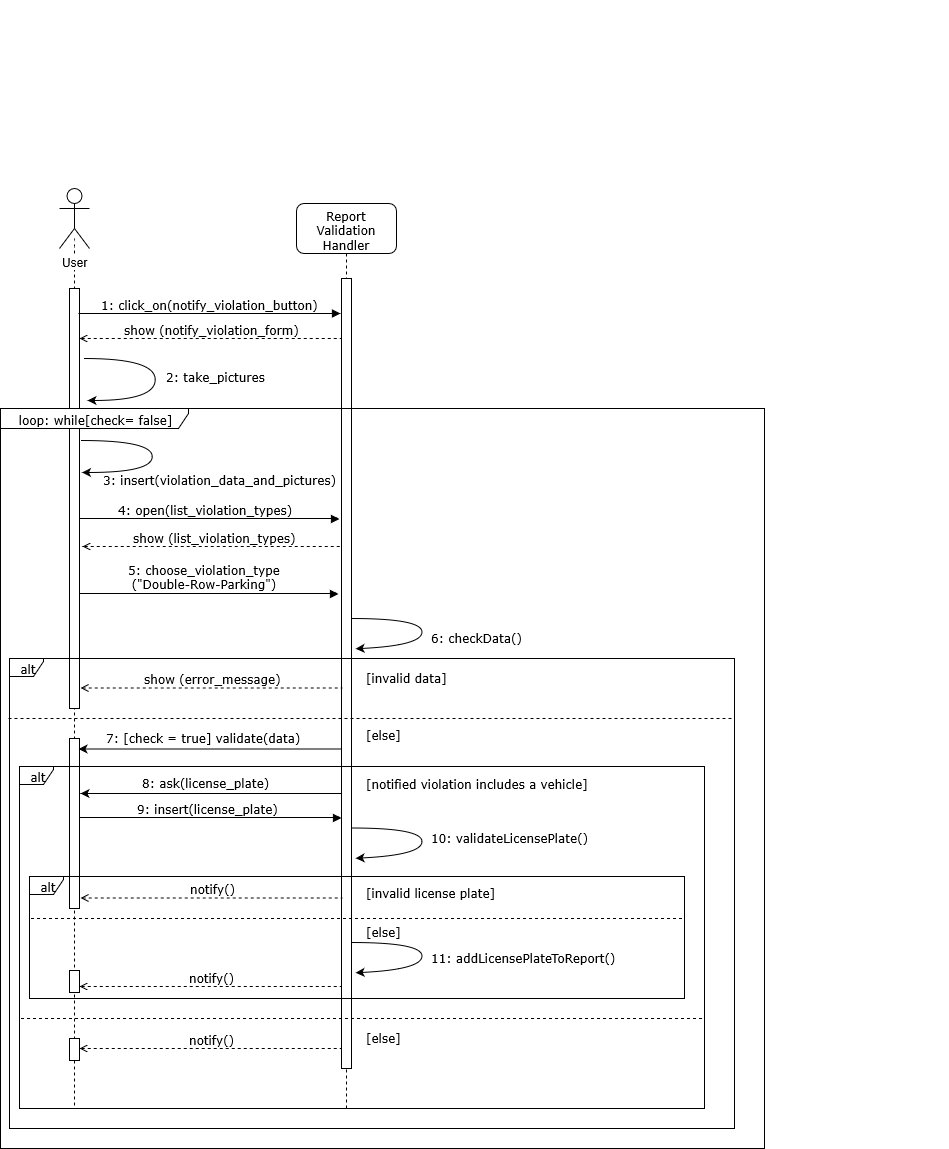
\includegraphics[width=\textwidth]{RASD_Images/SequenceDiagrams/2.jpg}
    \caption{\textit{Sequence diagram 2 - User sends pictures on mobile phone to notify a parking violation}}
\end{figure}

\newpage
\subsection{R3: Validation of reported violations}
\begin{itemize}
    \item Whenever a violation is reported the system checks whether or not the license plate field has been filled
    \item If the license plate is present, to prevent multiple tickets from being generated, the system verifies if the same kind of violation has already been reported in the previous $h$ hours for the same vehicle
    \item If the same violation has already been reported in the previous $h$ hours the report is automatically discarded, otherwise it is sent to a group of $k$ SafeStreets users for validation
    \item Users who receive the notification about this approval process are then asked to approve, reject or declare themselves neutral about the report
    \item The report is validated if and only if the algebraic sum of approvals (+1), neutralities (0) and rejections (-1) is at least $v$
    \item Every user is supposed to respond, the system expects to receive $k$ answers
    \item If a user doesn't answer within a certain amount of time, their answer is considered neutral
\end{itemize}
\begin{description}
    \item \textbf{Scenario 3} \newline
        SafeStreets has received the report of Mario Rossi regarding a violation of double-row parking. To verify the violation, a notification is sent to $k$ users. The system receives the answers that the users gave to the validation request and makes the algebraic sum of approvals and rejections. The calculated sum is $m > v$, where $v$ is a threshold that guarantees a minimum number of approvals; as a consequence, the system validates the report and registers the violation.

    \item \textbf{Use case: The system validates a reported violation}
        \begin{center}
            \begin{tabular}{|p{3cm}|p{7cm}|}
                \multicolumn{2}{c}{\textbf{User sends pictures to notify violation}} \\
                \hline
                \textbf{Name} & Validation of violation  \\
                \hline
                \textbf{Actor} & $k$ users \\
                \hline
                \textbf{Goals} & R3 \\
                \hline
                \textbf{Entry conditions} & A violation must have been notified by a user \\
                \hline
                \textbf{Event flow} &
                \begin{enumerate}
                    \item A user send a violation report to SafeStreets
                    \item The system sends a request to a number $k$ of users
                    \item Users answer the poll
                    \item The system counts the answers and makes the algebraic sum $m$, considering that:
                    \begin{itemize}
                        \item +1 is a confirmation of the violation
                        \item 0 is an absent response or an agnostic report of the violation
                        \item -1 is a refusal of the violation 
                    \end{itemize}
                    \item The system compares the calculated sum with the memorized acceptance threshold value $v$
                    \begin{enumerate}
                        \item If $m > v$ the system validates and register the report
                        \item If $m \leq v$ and the sample of users was less then $g$ the report is discarded
                        \item If $m \leq v$ and the sample of users was greater or equal to $g$ the report is discarded and the user who submitted it receives a penalty
                    \end{enumerate}
                    % TODO: Manage penalty and fidelity points
                \end{enumerate} \\
                \hline
                \textbf{Exit conditions} & The system has validated and registered the violation \\
                \hline
                \textbf{Exceptions}
                & \begin{itemize}
                    \item Another violation report has already been sent in the previous $h$ hours with the same violation category and license plate
                \end{itemize} \\
                \hline
            \end{tabular}
        \end{center}
\end{description}

\begin{figure}[hbt!]
    \centering
    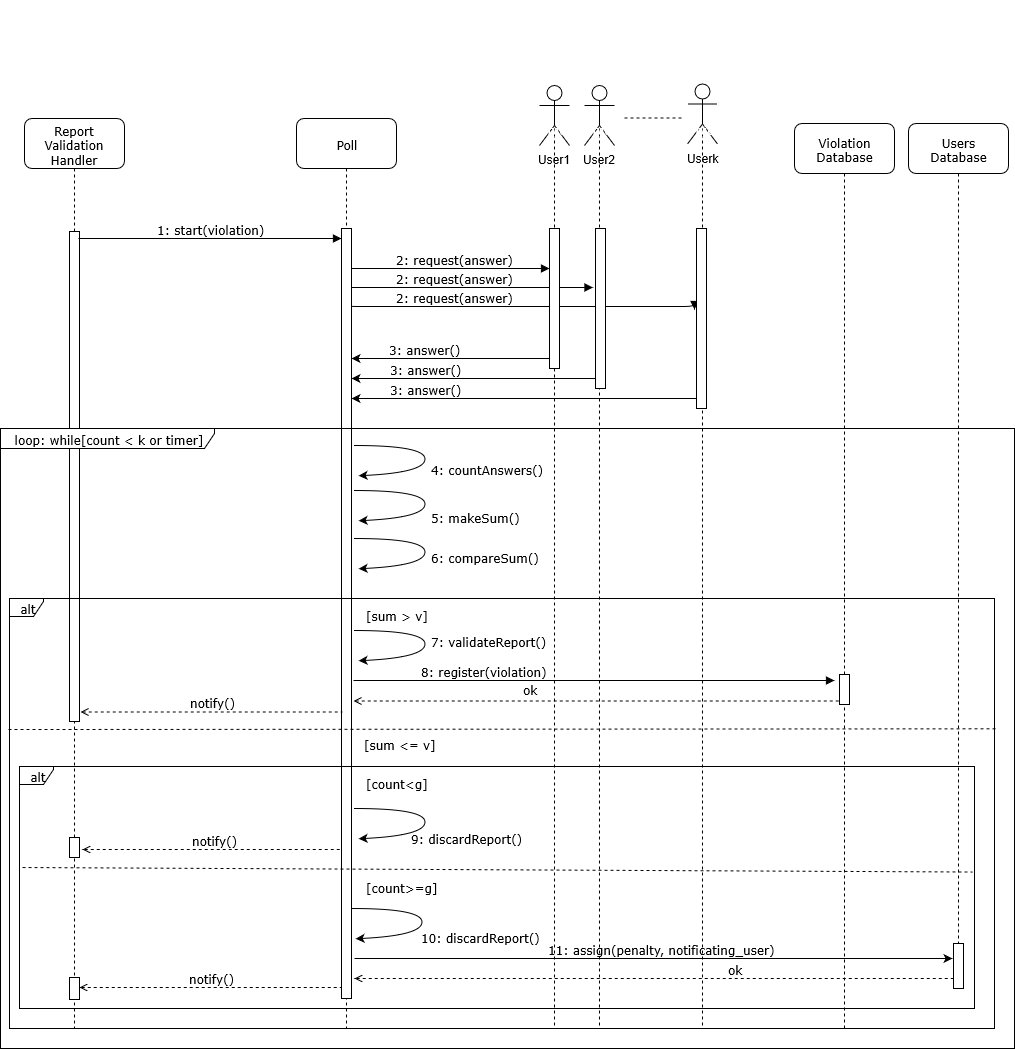
\includegraphics[width=\textwidth]{RASD_Images/SequenceDiagrams/3.jpg}
    \caption{\textit{Sequence diagram 3 - The system validates a reported violation}}
\end{figure}

\subsection{R4: Allow a user to see the areas where a violation is more likely to happen}
\begin{itemize}
    \item SafeStreets can aggregate data inputted by users to show relevant statistics about the frequency of traffic violations
    \item Users can see how many violations usually happen in their neighborhood, in their current location or in an area of their choice
    \item A user has access to the type and amount of violations that happened
    \item Users can insert a specific address to check
    \item The system answers showing the nearest unsafe areas, if the address is located in a safe area
    \item The system answers showing more detailed data about frequency of car accidents and violations, if the address is in an unsafe area
\end{itemize}

\begin{description}
    \item \textbf{Scenario 4} \newline
        Mario Rossi searches for an English school for his daughter, he founds different schools in his city on the Internet, but he wants an area 
        not too far from his house where the little girl can securely go also on foot. He has to decide among five schools. He is a user of SafeStreets, so 
        for every school in his list, he looks on the web interface of the application for the statistics about car accidents in all the five zones. He inserts the address of the school and the system responds with a map, showing the nearest unsafe areas if the school is in a safe area, or, if the school is in an unsafe 
        area, showing more detailed data about frequency of car accidents and violations. This operation is repeated five times.

    \item \textbf{Use case: User looks for statistics for unsafe areas}
        \begin{center}
            \begin{tabular}{|p{3cm}|p{7cm}|}
                \multicolumn{2}{c}{\textbf{User looks for statistics for unsafe areas}} \\
                \hline
                \textbf{Name} & Viewing of statistics \\
                \hline
                \textbf{Actor} & User \\
                \hline
                \textbf{Goals} & R4 \\
                \hline
                \textbf{Entry conditions} & The user must be registered to the application and he must have logged on the web interface\\
                \hline
                \textbf{Event flow} &
                \begin{enumerate}
                    \item The user clicks on the "View statistics" button
                    \item The user inserts the address he looks for
                    \item The system shows a map with the area surrounding the inserted address
                \end{enumerate} \\
                \hline
                \textbf{Exit conditions} & The user has seen the statistics he required \\
                \hline
                \textbf{Exceptions}
                & \begin{itemize}
                    \item The area has insufficient data to provide statistically significant information
                \end{itemize} \\
                \hline
            \end{tabular}
        \end{center}
\end{description}

\begin{figure}[hbt!]
    \centering
    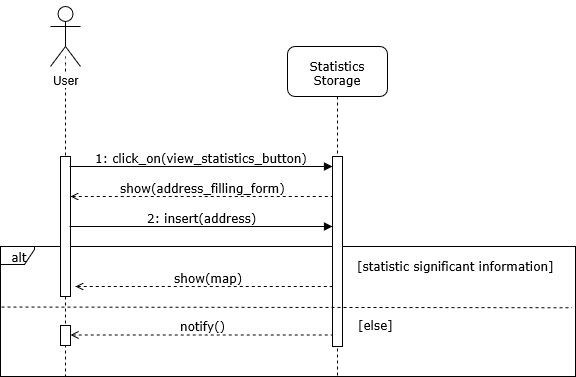
\includegraphics[width=\textwidth]{RASD_Images/SequenceDiagrams/4.jpg}
    \caption{\textit{Sequence diagram 4 - User looks for statistics for unsafe areas}}
\end{figure}

\newpage
\subsection{R5: Allow authorities to see data about violations and who committed them}
\begin{itemize}
    \item Authorities can access all data about violations that a standard user can access
    \item Authorities also have access to more specific data about who committed a violation, like the license plate of the car or how many infractions have been associated to a specific car
    \item In case the validated report includes a vehicle and the license plate is correctly identified, the authority can generate a traffic ticket
\end{itemize}
\begin{description}
    \item \label{scenario5} \textbf{Scenario 5} \newline
        A notification of a violation including a vehicle has just been made by a registered user and has been validated. The type of violation is "Stop in front of driveway" and the offender car, that has been identified with its license plate, was already present in the list SafeStreets uses to keep track of offenders. The system updates the number of infractions related to that car. An authority views the new infraction and generate a traffic ticket. The authority is also able to see the history of violations regarding the offender.

    \item \textbf{Use case: Viewing of data about violations and offenders by authorities}
    \begin{center}
        \begin{tabular}{|p{3cm}|p{7cm}|}
            \multicolumn{2}{c}{\textbf{Viewing of data about violations and offenders by authorities}} \\
            \hline
            \textbf{Name} & An authority sees offenders profile and data \\
            \hline
            \textbf{Actor} & Authority \\
            \hline
            \textbf{Goals} & R5 \\
            \hline
            \textbf{Entry conditions} & A notification, including a vehicle, must have been made, validated and registered.
            The system has identified the license plate of the offender. \\
            \hline
            \textbf{Event flow} &
            \begin{enumerate}
                \item The system updates the number of violations associated to that vehicle
                \item The authority checks the history of violation related to the offender
                \item The authority generates a traffic ticket
            \end{enumerate} \\
            \hline
            \textbf{Exit conditions} & The authority handled a violation report \\
            \hline
            \textbf{Exceptions}
            & \begin{itemize}
                \item The license plate of the offender is not identified
            \end{itemize} \\
            \hline
        \end{tabular}
    \end{center}
\end{description}

\begin{figure}[hbt!]
    \centering
    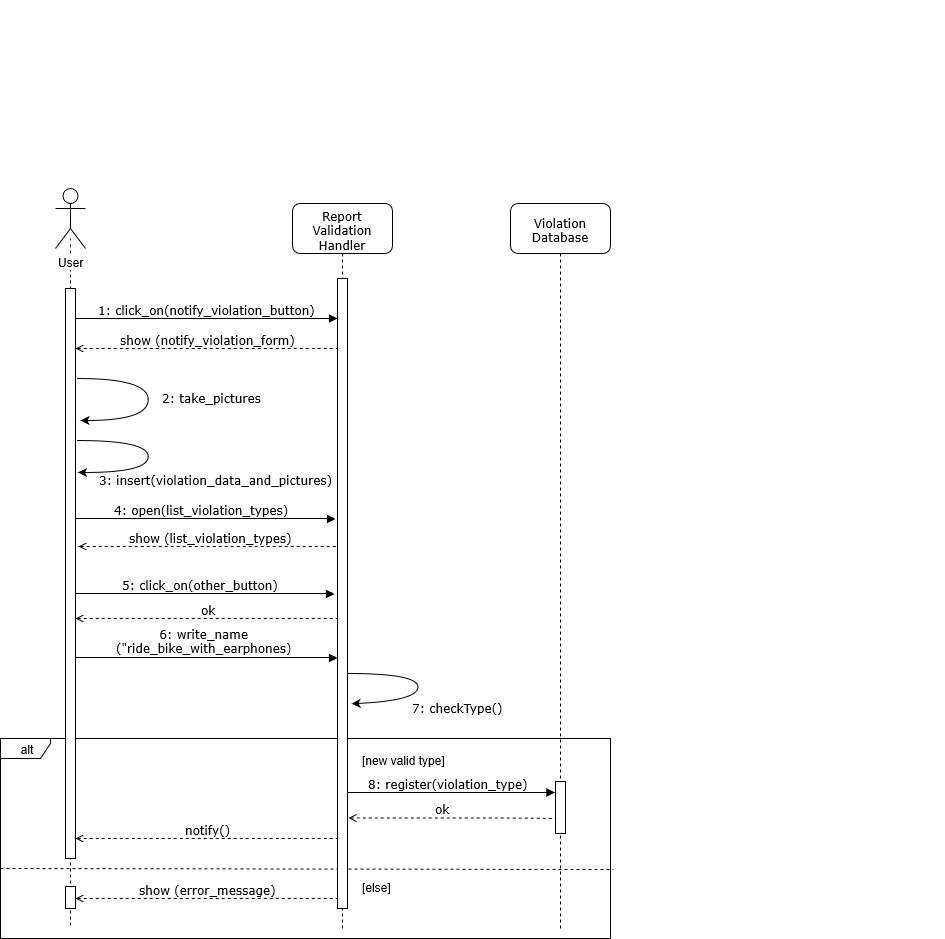
\includegraphics[width=\textwidth]{RASD_Images/SequenceDiagrams/5.jpg}
    \caption{\textit{Sequence diagram 5 - Viewing of data about violations and offenders by authorities}}
\end{figure}

\newpage
\subsection{R6: Allow authorities to register with a special user profile}
\begin{itemize}
    \item Authorities must first register as citizens
    \item A standard user profile can be upgraded to an authority profile if it is verified by the system
    \item To obtain privileged access, the user must provide a valid document that proves their authority status
\end{itemize}
\begin{description}
    \item \textbf{Scenario 6} \newline
        Paolo Brambilla is a policeman, he wants to register to SafeStreets and using his tablet he accesses the web interface, inserts his data for standard user registration \hyperref[scenario1]{(see Scenario 1)} and becomes a registered user. He wants to upgrade his profile to be enabled, as a member of the local police, to access the most advanced functions of the system. He must click on the button "Upgrade profile", then he is asked to write his police ID badge number and his current district, then he clicks on the button "Upgrade to authority". The system verifies his ID badge number, sending it to the municipality that confirms or discards the identification of the policeman, checking his personal data, his area of competence and his badge. If the authority identity is validated, the profile is correctly upgraded. An confirmation email of the upgrade is sent to Paolo Brambilla's address. Now he can log to SafeStreets as an authority and has access to all the advanced functions of the system. If the authority identity is rejected, the system doesn't change anything in the user profile.

    \item \textbf{Use case: User registers as an authority}
    \begin{center}
        \begin{tabular}{|p{3cm}|p{7cm}|}
            \multicolumn{2}{c}{\textbf{Registration of an authority}} \\
            \hline
            \textbf{Name} & Registration of an authority \\
            \hline
            \textbf{Actor} & User/Authority \\
            \hline
            \textbf{Goals} & R6 \\
            \hline
            \textbf{Entry conditions} & The user must be registered to the application and he must have logged in \\
            \hline
            \textbf{Event flow} &
            \begin{enumerate}
                \item The user clicks on the "Upgrade profile" button
                \item The system asks to insert data for proving their authority role 
                \item The user inserts the police ID badge number and their district 
                \item The user clicks on the "Upgrade to authority" button
                \item The system sends data to municipality
                \item The municipality validates data 
                \item The system saves the authority's data and upgrades the user profile to authority level 
                \item The system sends a confirmation email
            \end{enumerate} \\
            \hline
            \textbf{Exit conditions} & The user has become an authority \\
            \hline
            \textbf{Exceptions}
            & \begin{itemize}
                \item The inserted district is not valid
                \item The police ID badge is already registered             
                \item The police ID badge is not valid
            \end{itemize} \\
            \hline
        \end{tabular}
    \end{center}
\end{description}

\begin{figure}[hbt!]
    \centering
    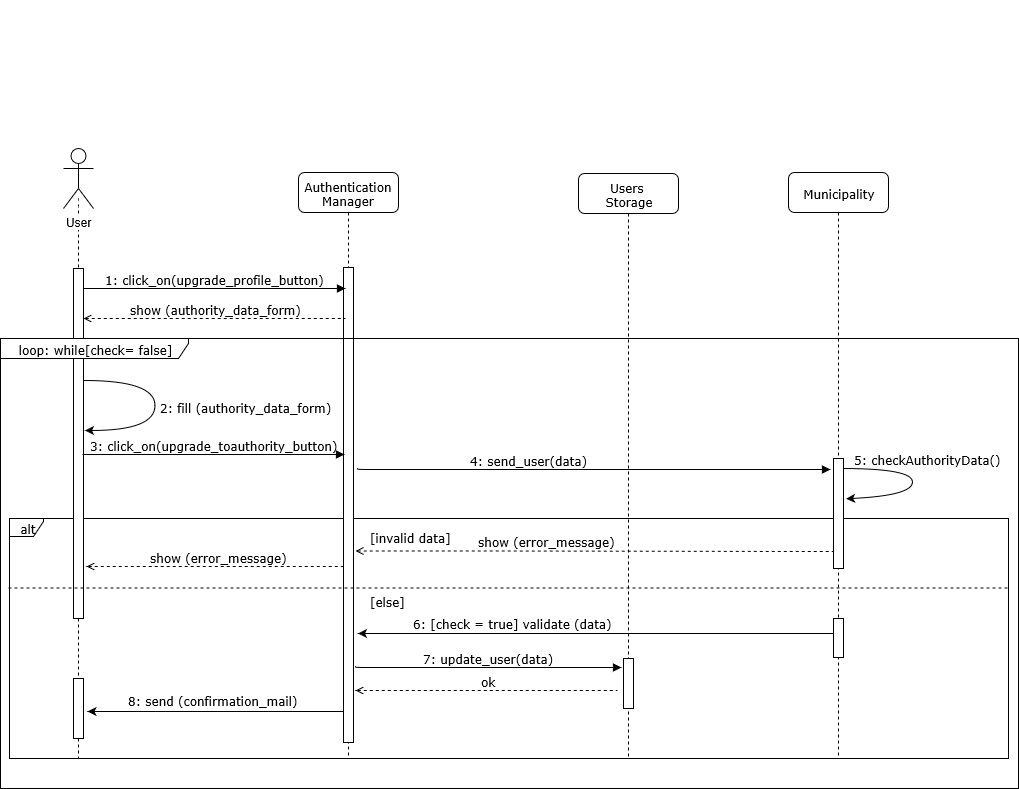
\includegraphics[width=\textwidth]{RASD_Images/SequenceDiagrams/6.jpg}
    \caption{\textit{Sequence diagram 6 - User registers as an authority}}
\end{figure}

\newpage
\subsection{R7: Detection of unsafe areas and possible interventions}
\begin{itemize}
  \item SafeStreets can cross information from different sources to identify potentially unsafe areas
  \item SafeStreets may be integrated with a public service, offered by the municipality, that provides such information
  \item Once identified, SafeStreets can suggest possible interventions to prevent accidents
\end{itemize}
\begin{description}
    \item \textbf{Scenario 7} \newline
        The system uses its own data, collected with reports of violation, and has the possibility to ask the municipality data about car 
        accidents and violations in a specific area. This information is crossed to SafeStreets that integrates the given data with the information
        already saved and verified. In this way the storage keeps track of the unsafe areas, that are identified as those with violations notified
        by SafeStreets users, those with car accidents and damages provided by the municipality, and those areas that have both these 
        information. On a regular basis, SafeStreets sends an email to the municipalities that can intervene on unsafe areas suggesting possible solutions identified using a special algorithm.
        
    \item \textbf{Use case: The system provides unsafe areas identification}
    \begin{center}
        \begin{tabular}{|p{3cm}|p{7cm}|}
            \multicolumn{2}{c}{\textbf{Unsafe areas identification}} \\
            \hline
            \textbf{Name} & Unsafe areas identification \\
            \hline
            \textbf{Actor} & SafeStreets Server \\
            \hline
            \textbf{Goals} & R7 \\
            \hline
            \textbf{Entry conditions} &  The system must select a specific area to identify\\
            \hline
            \textbf{Event flow} &
            \begin{enumerate}
                \item The system queries verified and validated reports of SafeStreets about the selected area
                \item $v$ violations are returned from reports
                \item The system queries municipality about car accidents in the selected area
                \item $a$ accidents are provided by the municipality
                \item The system determines unsafe areas by testing the equation $v + a > 0$ on the registered areas
                \item Periodically, the system sends an email containing possible solutions to the municipalities that can intervene on the unsafe areas identified
            \end{enumerate} \\
            \hline
            \textbf{Exit conditions} & New statistics have been saved by the system \\
            \hline
        \end{tabular}
    \end{center}
\end{description}

\begin{figure}[hbt!]
    \centering
    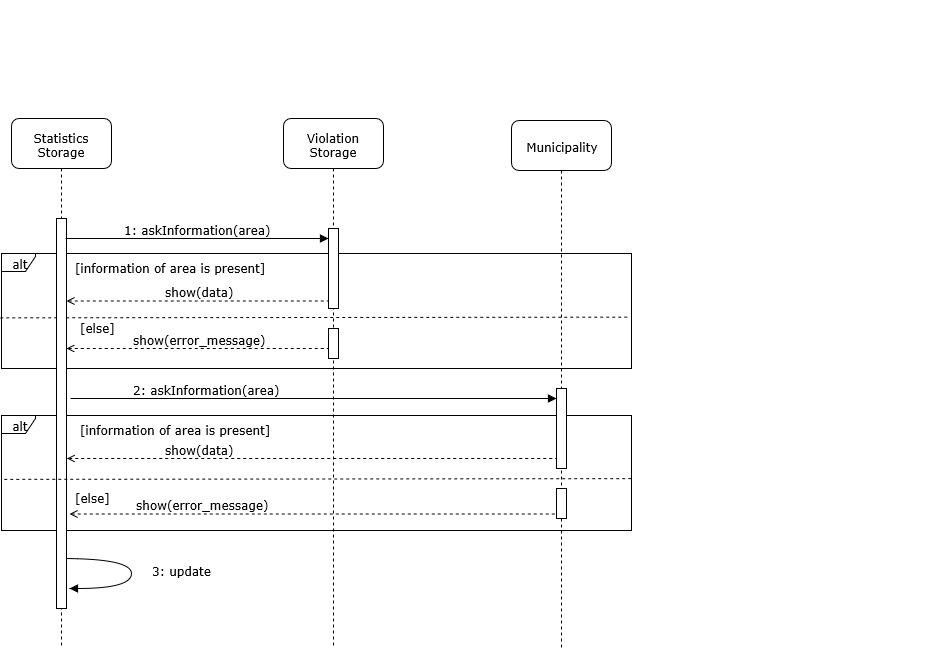
\includegraphics[width=\textwidth]{RASD_Images/SequenceDiagrams/7.jpg}
    \caption{\textit{Sequence diagram 7 - The system provides unsafe areas identification}}
\end{figure}

\newpage
\subsection{R8: Traffic ticket generation from validated reports}
\begin{itemize}
  \item SafeStreets can generate tickets for traffic violations reported from registered users
  \item The information is kept safe and intact through the chain of custody, from the end user to the local police officer issuing the tickets
\end{itemize}
\begin{description}
    \item \textbf{Scenario 8} \newline
        The information about the reports is stored in a database where privileges about the creation and modification of the information
        are distinct. Both the web interface and the mobile application can create new reports, only system administrators have full access to
        the database and thus it's their responsibility to guarantee that other actors don't alter the data. These conditions are necessary to allow SafeStreets tickets to have legal validity, thus enabling local authorities to automatically generate traffic ticket from the client application.
 
    \item \textbf{Use case: An authority provides municipality of information and traffic ticket is generated}
    \begin{center}
        \begin{tabular}{|p{3cm}|p{7cm}|}
            \multicolumn{2}{c}{\textbf{A traffic ticket is generated}} \\
            \hline
            \textbf{Name} & A traffic ticket is generated \\
            \hline
            \textbf{Actor} & Authority \\
            \hline
            \textbf{Goals} & R8 \\
            \hline
            \textbf{Entry conditions} & A violation has been approved \\
            \hline
            \textbf{Event flow} &
            \begin{enumerate}
                \item The system creates new records in the database regarding the reported violation
                \item Authorities can access report data in read-only mode
                \item Through the web interface an authority can automatically generate a standard ticket, filling out the missing information
            \end{enumerate} \\
            \hline
            \textbf{Exit conditions} & Traffic ticket is generated \\
            \hline
            \textbf{Exceptions}
            & \begin{itemize}
                \item A system administrator broke the chain of custody
            \end{itemize} \\
            \hline
        \end{tabular}
    \end{center}
\end{description}

\begin{figure}[hbt!]
    \centering
    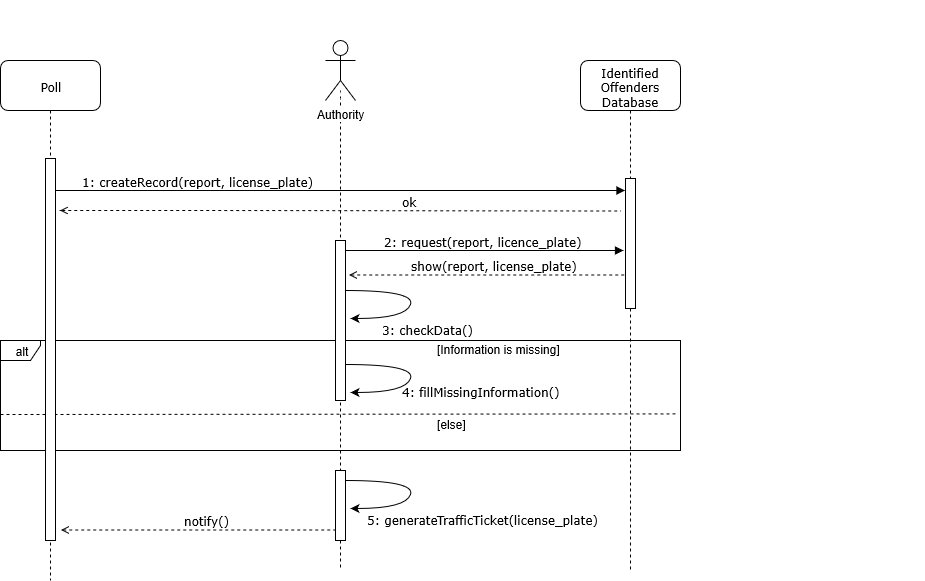
\includegraphics[width=\textwidth]{RASD_Images/SequenceDiagrams/8.jpg}
    \caption{\textit{Sequence diagram 8 - An authority provides municipality of information and traffic ticket is generated}}
\end{figure}

\newpage
\subsection{Traceability Matrix}
\begin{center}
    \begin{tabular}{c|c|l|l}
        \hline
        \textbf{Ref} & \textbf{Goals} & \textbf{Requirement} & \textbf{Domain assumptions} \\
        \hline
        1 & G1 & R1, R2 & D1, D5 \\
        \hline
        2 & G2 & R4, R7 & D8, D10 \\
        \hline
        3 & G3 & R5, R8 & D7, D9 \\
        \hline
        4 & G4 & R3 & D9, D11 \\
        \hline
        5 & G5 & R1, R6 & D2, D3, D6 \\
        \hline
        6 & G6 & R5, R8 & D1, D2 \\
        \hline
        7 & G7 & R1, R3, R5, R6, R8 & D1, D4, D5, D9, D11  \\
        \hline
    \end{tabular}
\end{center}
To improve readability, here is a brief description of the goals and the related requirements and domain assumptions. 
\begin{enumerate}
    \item The goal is to allow citizens of legal age to report violations. This means that citizens should be allowed to register providing a document to confirm their age and identity and then SafeStreets should allow them to submit pictures along with a report.
    \item The goal is to show statistics about the safety of different areas, and possibly offer some suggestions to make the worst areas safer. The statistics are going to be more reliable if the municipalities allow SafeStreets to access their data about violations, but still the safety of an area is computed only using previous data and its accuracy is strictly dependent on the amount of reports that SafeStreets has access to.
    \item The goal is to show the violations to the authorities, in order to enable them to take action. This means that SafeStreets must have a way to verify that a user is actually an authority, because only authorities are allowed to generate traffic tickets.
    \item The goal is to validate reports through a reliable procedure. This means that after a report is sent, it can't be modified.
    \item The goal is to provide secure authentication methods, for example by allowing two-factors authentication.
    \item The goal is to securely store user data and make it available only to authorized people.
    \item The goal is to give legal validity to approved violation reports, so that tickets can be generated: only users with a verified profile and who are of legal age are allowed to submit reports, and once generated, a report can't be altered.
\end{enumerate}